%Observação importante: para usar os recursos da classe ABNTEX, é necessário fazer o download de sua biblioteca,
%visto que a mesma não é nativa do ambiente \LaTeX.
%Em um distribuição linux baseada em debian o pacote pode ser instalado pelo comando: sudo apt-get install abntex.
%Autor:Jean Henrique Ferreira Freire

\documentclass{abnt}
\usepackage[brazil]{babel}
\usepackage[utf8]{inputenc}
\usepackage[num]{abntcite}
\usepackage{graphicx}
\usepackage{amsthm}
\usepackage{url}

\begin{document}
\autor{Vitor Botelho Vaz de Melo}

\titulo{Identificando Linhas de Códigos Comentadas em Repositórios de Software}

\orientador[Orientador:\\]{André Hora - Departamento de Ciência da Computação}




\comentario{Proposta de Projeto de Pesquisa e Tecnológico da disciplina de Projeto Orientado em Computação do DCC/UFMG}

\instituicao{Universidade Federal de Minas Gerais \par Instituto de Ciências
Exatas \par Departamento de Ciência da Computação}

\local{Belo Horizonte} \data{2019/2}

% \capa 

\folhaderosto 


% \begin{resumo}
% Coloque aqui seu resumo.\\


% \textbf{Palavras-chaves}: palavras, chave. 
% \end{resumo}

% \sumario %comando que gera o sumário automaticamente
% \renewcommand*\listfigurename{LISTA DE FIGURAS}
% \listoffigures %comando que gera um sumário para a lista de figuras do texto automaticamente



\chapter{INTRODUÇÃO}


À medida que a Ciência da Computação avança e milhões de linhas de códigos são 
escritas, diariamente e em diversas linguagens de programação, os desenvolvedores 
percebem que, para alcançar sucesso a médio e longo prazo em seus projetos, é
necessário utilizar-se, cada vez mais, das melhores ferramentas e práticas de 
programação. 

Uma prática de programação muito comum ao se desenvolver softwares é a de 
''remover'' uma linha ou um bloco de código tornando-os comentários, sendo conhecida  
como \textit{commented-out code} (Figura \ref{fig:commentExample}). Remover uma linha de código 
por comentário pode ser útil, tanto que 
os próprios ambientes de programação (IDE's e editores de texto) oferecem atalhos 
fáceis para isso. Contudo, esta prática se torna um verdadeiro problema quando 
estes códigos comentados estão inseridos em um sistema grande, complexo e
mantido por diversas pessoas.\cite{cleanCode}.

\begin{figure}[h!]
  \centering
  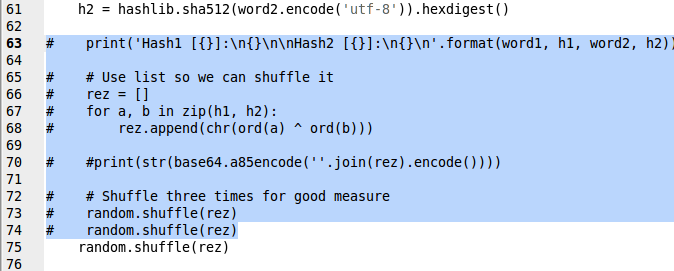
\includegraphics[height=2.4in,width=6.3in]{../images/gcc06.png}
  \caption{Commented-out code example }
  \label{fig:commentExample}
\end{figure}


A inserção de código comentado nos arquivos fontes de um sistema pode causar
redução da legibilidade, distração e perda de tempo. MARTIN R., em seu livro clássico
Clean Code, enfatiza \textit{Few practices are as odious as commenting-out code. 
Don’t do this!}, ele argumenta que outras pessoas não terão coragem de deletar 
este código por achar que ele pode ser importante~\cite{cleanCode}. 

Além disso, quando um mantenedor se depara com códigos comentados ele pode ter uma 
série de dúvidas, como \textit{"Por que este código está comentado? Isso é útil em 
alguma função? Este código está relacionado com determinada mudança?"}, entre outras 
questões específicas para cada sistema. Este tipo de reflexão pode no mínimo ser 
uma perda de tempo, ou até mesmo uma distração para introduzir bugs no sistema \cite{cleanCode}.

Na disciplina Projeto Orientado em Computação I foi desenvolvida uma ferramenta
apropriada para identificar \textit{commented-out code} utilizando técnicas de aprendizado de máquina.
Portanto, na disciplina Projeto Orientado em Computação II será realizado um estudo abrangente desta 
prática em diversos repositórios de código aberto.


\chapter{REFERENCIAL TEÓRICO}


\section{Trabalhos Anteriores}

GRIJÓ L. e HORA A. exploraram o problema da inserção de código comentado 
e demostraram interessantes resultados no artigo Minerando Código Comentado 
\cite{articleMiningComments}. No trabalho foi desenvolvido um parser heurístico
que identifica \textit{commented-out code} para a linguagem java que, e obteve
uma precisão de 83\%. Com esta ferramenta foi identificado que alguns 
sistemas possuem como mediana 4,17\% de taxa de commented-out code em relação
ao total de comentários, com alguns sistemas chegando a 30\%.


\section{Mineração de Repositórios de Software}

Para se entender as práticas e diversas informações sobre um sistema pode-se
analisar as diferentes versões do código deste sistema. Dessa forma pode-se 
identificar em um sistema as boas e más práticas presentes, questões arquiteturais,
entre outras questões, com o objetivo de melhorar a manutenibilidade deste sistema.
Através da mineração de repositório de software podemos 
predizer quais seções do código apresentam mais defeitos e maior
dificuldade de compreensão; usar a evolução do software para identificar
partes do código que são mais importantes para manutenção; entender como diversos
desenvolvedores e times afetam a qualidade do código.
\cite{crimeScene}. 


\section{Git e GitHub}

Git\footnote{https://git-scm.com/} é uma ferramenta amplamente usada na 
comunidade de desenvolvimento de software para controle de versão de código.
Ela permite que seja avaliado diferentes versões do código de um mesmo 
sistema~\cite{articleMiningGit}. O Github\footnote{https://github.com/} é 
uma plataforma que permite hospedar repositórios de código com o sistema de versionamento
Git na nuvem. Nele é possível encontrar diversos repositórios de código aberto 
que serão as fontes de estudo deste trabalho. 

\section{Algoritmos de Classificação}
Os algoritmos de classificação são algoritmos de aprendizado supervisionado,
no qual utilizamos uma base de treino em que previamente sabemos a "classe" 
de cada objeto para treinar um modelo que pode dizer qual a classe dos 
objetos dos quais não conhecemos \cite{patternClassification}.

Podemos modelar o problema de identificar \textit{commented-out code} como sendo um problema
de classificação binária. Neste caso, os objetos serão os comentários presentes em 
códigos de diversas linguagens, e a classe será se aquele comentário é normal 
representado por 0 ou código comentado representado por 1.

\subsection{Precisão e Revocação}
As taxas de precisão (\textit{precision}) e revocação (\textit{recall}) nos permite avaliar a qualidade do classificador~\cite{powers2011evaluation}.
Elas são definidas como:
\begin{center}
  

\begin{math}
  precision = \frac{tp}{tp +fp}
\end{math}~~~~~
\begin{math}
  recall = \frac{tp}{tp +fn}
\end{math}
\end{center}

\begin{itemize}
  \item tp = True Positive: Elementos classificados como 1 ou positivos corretamente.
  \item fp = False Positives: Elementos classificados como 1 ou positivos incorretamente.
  \item fn = False Negative: Elementos classificados como 0 ou negativos incorretamente.
\end{itemize}


\chapter{METODOLOGIA}


\section{Construção de um pipeline de execução }

Na disciplina de Projeto Orientado em Computação I foram criadas duas principais ferramentas,
A primeira separa um arquivo "completo" de código em código e comentário. A segunda identifica,
dentro dos comentários, o que seria \textit{commented-out code}. Além disso, há bibliotecas 
para o Git e GitHub que permitem caminhar via software por diversas versões de um repositório.

Portanto será criada uma ferramenta que integra todas as etapas necessárias para
a coleta de informações relativas a esta prática em diferentes versões de diversos 
repositórios de software.

\begin{figure}[h!]
  \centering
  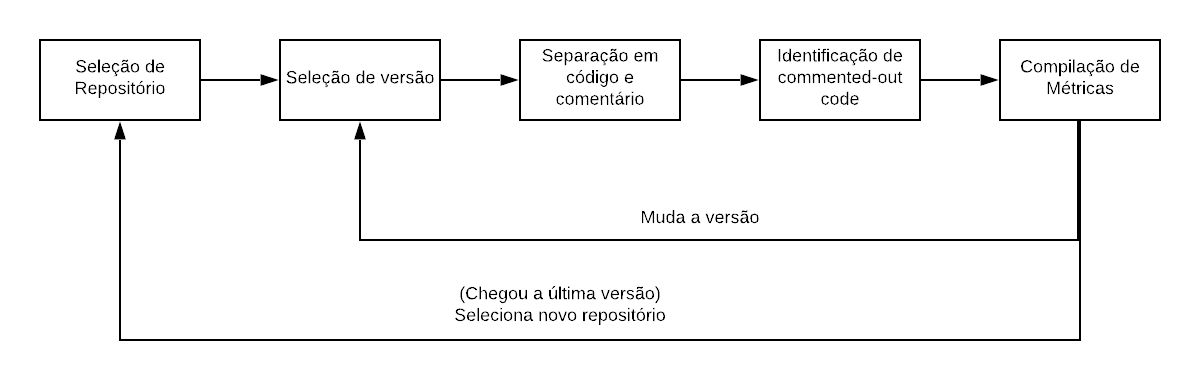
\includegraphics[height=2.4in,width=6.3in]{../images/pipeline-flow.png}
  \caption{Fluxo de execução do algoritmo}
  \label{fig:commentExample}
\end{figure}


\section{Compilação de dados de Repositórios}

Com a ferramenta preparada, serão analisados 
diversos repositórios relevantes de softwares de código aberto, encontrados
no GitHub. Ao identificar os comentários, será possível calcular a taxa de 
código comentado em relação ao total de comentários em uma versão do 
software, e com o auxilio da ferramenta Git será analisado a evolução do 
software através do código em diferentes versões. Com isso teremos 
indícios de como os desenvolvedores estão lidando com essa prática, entre 
diversas outras informações que podem ser exploradas com este tipo
de técnica.

\chapter{RESULTADOS ESPERADOS}

Ao final da disciplina Projeto Orientado em Computação I  foi
obtida uma ferramenta robusta e com alto nível de precisão para identificar 
códigos comentados em diversas linguagens de programação. No final da 
disciplina Projeto Orientado em Computação II espera-se compreender como a 
má prática de remover código através de comentário afeta a evolução dos 
diferentes repositórios de código aberto, respondendo perguntas como:
\textbf{(1)} Qual a taxa de código comentado média nos repositórios de software?
\textbf{(2)} Como essa taxa evolui ao longo das versões.
\textbf{(3)} Ela varia dependendo da linguagem?
\textbf{(4)} Existe uma correlação entre arquivos mais modificados e a presença de 
    código comentado?,
dentre outras questões.



\chapter{ETAPAS E CRONOGRAMAS}

\begin{table}[ht]
  \centering
  \label{tab:Table1}
  \smallskip
  \begin{tabular}{cp{11cm}}
  Período & Atividade\\[0.5ex]
  \hline
  11/08 a 08/09 & Consolidação do POC I e elaboração de proposta para o POC II \\[0.5ex]

  09/09 a 29/09 & Criação do pipeline de execução.\\[0.5ex]
  
  30/09 a 04/10 & Elaboração e Apresentação intermediária. \\[0.5ex]

  05/10 a 20/10 & Execução do algoritmo em diversos repositórios de software  \\[0.5ex]

  21/10 a 10/11 & Visualização e análise dos dados coletados \\[0.5ex]

  11/11 a 05/12 & Elaboração do artigo, poster e apresentação final. \\[0.5ex]
  \end{tabular}
  \end{table}

\bibliography{references.bib}

\end{document}
